 \documentclass[12pt]{article}
 
\usepackage[margin=1in]{geometry} 
\usepackage{amsmath,amsthm,amssymb}
\usepackage{pgfplots}
\usepackage{float}
 
\newcommand{\N}{\mathbb{N}}
\newcommand{\Z}{\mathbb{Z}}
 
\newenvironment{theorem}[2][]{\begin{trivlist}
\item[{\bfseries #1}\hskip \labelsep {\bfseries #2.}]}{\end{trivlist}}
\newenvironment{lemma}[2][Lemma]{\begin{trivlist}
\item[\hskip \labelsep {\bfseries #1}\hskip \labelsep {\bfseries #2.}]}{\end{trivlist}}
\newenvironment{exercise}[2][Exercise]{\begin{trivlist}
\item[\hskip \labelsep {\bfseries #1}\hskip \labelsep {\bfseries #2.}]}{\end{trivlist}}
\newenvironment{reflection}[2][Reflection]{\begin{trivlist}
\item[\hskip \labelsep {\bfseries #1}\hskip \labelsep {\bfseries #2.}]}{\end{trivlist}}
\newenvironment{proposition}[2][Proposition]{\begin{trivlist}
\item[\hskip \labelsep {\bfseries #1}\hskip \labelsep {\bfseries #2.}]}{\end{trivlist}}
\newenvironment{corollary}[2][Corollary]{\begin{trivlist}
\item[\hskip \labelsep {\bfseries #1}\hskip \labelsep {\bfseries #2.}]}{\end{trivlist}}
\theoremstyle{remark}
\newtheorem*{remark}{Remark}
 
\begin{document}
 
%\renewcommand{\qedsymbol}{\filledbox}
 
\title{Homework 3}
\author{David Miller \\ 
MAP 5345: Partial Differential Equations I} 
 
\maketitle

\subsection*{Problem 1}

\textit{Consider the wave equation $u_{tt} = c^2u_{xx}$. D'Alembert's solution is $u(x,t) = f(x+ct) + g(x-ct)$ for any functions f and g that are twice differentiable.} \\

\noindent \textit{(a) Verify D'Alemberts solution directly by simply inserting it into the PDE.} \\ \\
Using D'Alembert's solution we get the following partials
\begin{align*}
\partial_{t}(f(x+ct) + g(x - ct)) & = \frac{\partial f}{\partial t} + \frac{\partial g}{\partial t} \\
& = \frac{\partial f}{\partial (x+ct)}\frac{\partial (x+ct)}{\partial t} + \frac{\partial g}{\partial (x-ct)}\frac{\partial (x-ct)}{\partial t} \\
& = cf^\prime(x+ct) - cg^\prime(x+ct) \\
\partial_{tt}(f(x+ct) + g(x+ct)) & = c(\frac{\partial f^\prime}{\partial t} - \frac{\partial g^\prime}{\partial t}) \\
& = c\bigg(\frac{\partial f^\prime}{\partial (x+ct)}\frac{\partial (x+ct)}{\partial t} - \frac{\partial g^\prime}{\partial (x-ct)}\frac{\partial (x-ct)}{\partial t}\bigg) \\
& = c^2f^{\prime\prime}(x+ct) + c^2g^{\prime\prime}(x-ct) \\
\partial_{x}(f(x+ct) + g(x - ct)) & = \frac{\partial f}{\partial x} + \frac{\partial g}{\partial x} \\
& = \frac{\partial f}{\partial (x+ct)}\frac{\partial (x+ct)}{\partial x} + \frac{\partial g}{\partial (x-ct)}\frac{\partial (x-ct)}{\partial x} \\
& = f^\prime(x+ct) + g^\prime(x+ct) \\
\partial_{xx}(f(x+ct) + g(x-ct)) & = \frac{\partial f^\prime}{\partial x} + \frac{\partial g^\prime}{\partial x} \\
& = \frac{\partial f^\prime}{\partial (x+ct)}\frac{\partial (x+ct)}{\partial x} + \frac{\partial g^\prime}{\partial (x-ct)}\frac{\partial (x-ct)}{\partial x} \\
& = f^{\prime\prime}(x+ct) + g^{\prime\prime}(x-ct)
\end{align*}
Plugging this into the PDE we get
\begin{align*}
c^2f^{\prime\prime}(x+ct) + c^2g^{\prime\prime}(x-ct) = c^2(f^{\prime\prime}(x+ct) + g^{\prime\prime}(x-ct)) \quad \checkmark
\end{align*}
\textit{(b) Now consider the 'free-space' initial value problem}
\begin{align*} 
& u_{tt} = c^2u_{xx} \quad \text{for } -\infty < x < \infty, t > 0 \\
& u(x,0) = \phi (x) \\
& u_t(x,0) = \psi (x) 
\end{align*}
\textit{Use D'Alembert's solution to solve the IVP and determine $f$ and $g$.} \\ \\
Using the initial conditions we get
\begin{align*}
& f(x) + g(x) = \phi (x) \\
& cf^\prime (x) - cg^\prime(x) = \psi (x) 
\end{align*}
Integrating the second 
\begin{align*}
& \int\limits_{x_0}^{x_f} \bigg(f^\prime(x) - g^\prime(x)\bigg) dx = \frac{1}{c}\int\limits_{x_0}^{x_f} \psi(x) dx \\
& f(x) = g(x) + \frac{1}{c}\int\limits_{x_0}^{x_f} \psi(x) dx \quad (*)
\end{align*}
Plugging this back into the initial conditions
\begin{align*}
& \underbrace{g(x) + \frac{1}{c}\int\limits_{x_0}^{x_f} \psi(x) dx}_{f(x)} + g(x) = \phi(x) \\
\Rightarrow & \boxed{g(x) = \frac{1}{2}\phi(x) - \frac{1}{2c}\int\limits_{x_0}^{x_f} \psi(x) dx}
\end{align*}
Plugging this back into $(*)$
\begin{align*}
& f(x) = \frac{1}{2}\phi(x) - \frac{1}{2c}\int\limits_{x_0}^{x_f} \psi(x) dx + \frac{1}{c}\int\limits_{x_0}^{x_f} \psi(x) dx \\
\Rightarrow & \boxed{f(x) = \frac{1}{2}\phi(x) + \frac{1}{2c}\int\limits_{x_0}^{x_f} \psi(x) dx}
\end{align*}

\newpage

\noindent \textit{(c) Set $c=1$ and consider the initial conditions}
\begin{align*}
& u(x,0) = e^{-x^2/2} \\
& u_t(x,0) = 0
\end{align*}
\textit{Determine the solution to this IVP. First, plot the solution by hand for a few time values, without the aid of a computer. Next, plot the solution with Julia (choose a reasonable $x$-interval) and verify your had plot.} \\ \\
From the initial conditions we have
\begin{align*}
& f(x) + g(x) = e^{-x^2/2} \\
& cf(x) - cg(x) = 0 \Rightarrow f(x) = g(x)
\end{align*}
Plugging the second into the first
\begin{align*}
& 2f(x) = 2g(x) = e^{-x^2/2} \\
& \Rightarrow f(x) = g(x) = \frac{1}{2}e^{-x^2/2}
\end{align*}
Plugging this into D'Alembert's formula we get
\begin{align*}
& u(x,t) = f(x+ct) + g(x-ct) \\
\Rightarrow & \boxed{u(x,t) = \frac{1}{2}\bigg(e^{-(x+ct)^2/2}  + e^{-(x-ct)^2/2}\bigg)}
\end{align*}

\begin{figure}[H]
\centering
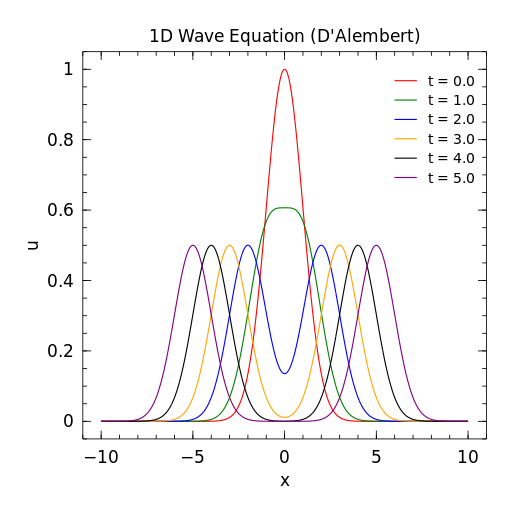
\includegraphics[width=10cm]{HW3_1c.png}
\end{figure}

\vphantom{}\vspace{7cm}

\noindent \textit{(d) Do the same for the initial conditions}
\begin{align*} 
& u(x,0) = 0 \\
& u_t(x,0) = xe^{-x^2/2}
\end{align*}
From the initial conditions we have
\begin{align*}
& f(x) + g(x) = 0 \Rightarrow f(x) = -g(x) \\
& cf^\prime(x) - cg^\prime(x) = xe^{-x^2/2}
\end{align*}
Plugging the first into the second
\begin{align*}
& 2cf^\prime(x) = xe^{-x^2/2}
\end{align*}
Integrating both sides we get
\begin{align*}
& \int\limits_{x_0}^{x_f} f^\prime(x) dx = \frac{1}{2c}\int\limits_{x_0}^{x_f} xe^{-x^2/2} dx \\
\Rightarrow & f(x) = -\frac{1}{2c}\bigg(e^{x_f^2/2} - e^{x_0^2/2}\bigg), \quad g(x) = \frac{1}{2c}\bigg(e^{x_f^2/2} - e^{x_0^2/2}\bigg)
\end{align*}
Plugging this back into D'Alembert's formula we get
\begin{align*}
& u(x,t) = f(x+ct) + g(x-ct) \\
& u(x,t) = -\frac{1}{2c}\bigg(e^{(x+ct)^2/2} - e^{x_0^2/2}\bigg) + \frac{1}{2c}\bigg(e^{(x-ct)^2/2} - e^{x_0^2/2}\bigg) \\
\Rightarrow & \boxed{u(x,t) = \frac{1}{2c}\bigg(e^{(x-ct)^2/2} - e^{(x+ct)^2/2}\bigg)} 
\end{align*}

\begin{figure}[H]
\centering
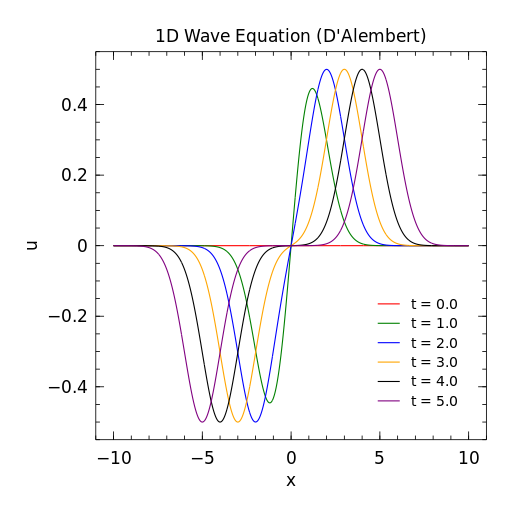
\includegraphics[width=10cm]{HW3_1d.png}
\end{figure}

\newpage

\subsection*{Problem 2 INCOMPLETE :(}

\textit{Now consider the vibrating string with clamped ends, given by th IBVP}
\begin{align*}
& u_{tt} = c^2u_{xx} \quad \text{for } 0 < x < L, t > 0 \\
& u(x,0) = \phi(x) \\
& u_t(x,0) = \psi(x) \\
& u(0,t) = u(L,t) = 0 
\end{align*}
\textit{Consider a relatively simple case in which $\phi(x) = x(L-x)$ and $\psi(x) = 0$.} \\ \\
\textit{(a) Can you use D'Alembert's formula to construct the exact solution to this problem?} \\ \\
Yes, we can use D'Alembert's formula to construct the exact solution to this problem. \\ \\
Using the boundary conditions we get 
\begin{align*}
& f(ct) + g(-ct) = 0 \Rightarrow f(ct) = - g(-ct) \\
& f(L+ct) + g(L-ct) = 0 \Rightarrow f(L+ct) = -g(L-ct)
\end{align*}
If we let $a = L + ct$ we get
\begin{align*}
& f(a) = -g(2L-a) \text{ and } f(ct) = -g(-ct)
\end{align*}
from this we can conclude some useful functions. For arbitrary values $s$ we get that
\begin{align*}
f(s) = -g(-s) \quad \text{ and } \quad f(s) = -g(2L-s)
\end{align*}
From these two equations we can determine $f$ on the entire real line! This is done by the following
\begin{align*}
f(s) & = f(s) \quad && \text{for } 0 \leq s \leq L \\
f(s) & = -g(2L-s) \quad &&  \text{for } L \leq s \leq 2L \\
f(s) & = -g(2L-s) = f(s-2L) \quad && \text{for } 2L\leq s \leq 3L \\
f(s) & = -g(2L-s) = f(s-2L) = -g(4L - s) \quad && \text{for } 3L \leq s \leq 4L \\
& \vdots && \vdots
\end{align*}
The same can be done for $g$ but on the domain $(-\infty,0]$. Doing so we have constructed a $u(x,t)$ that satisifies both the boundary conditions in the entire real line. \\ \\
\textit{(b) Using Julia, plot the solution for several time values. You solved the exact same IBVP in HW 2 using separation of variables. Compare your two solutions and make sure they are nearly the same. Is one more accurate than the other?} \\ \\
D'Alembert's formula is more accurate than the seperation of variables solution because their is no truncation. For the seperation of variables gneneral soulution we must pick some value $N$ that we truncate the infinite sum, effectively losing precision, where as D'Alembert's formula is an exact solution. 



\end{document}